%!TEX TS-program = xelatex
% Исходная версия шаблона --- 
% https://www.writelatex.com/coursera/latex/5.1
\documentclass[c, dvipsnames]{beamer}  % [t], [c], или [b] --- вертикальное 
%\documentclass[handout, dvipsnames, c]{beamer} % Раздаточный материал (на слайдах всё сразу)
%выравнивание на слайдах (верх, центр, низ)
%\documentclass[handout, dvipsnames]{beamer} % Раздаточный материал (на слайдах всё сразу)
%\documentclass[aspectratio=169, dvipsnames]{beamer} % Соотношение сторон
\setbeamertemplate{navigation symbols}{}%remove navigation symbols

%\usetheme{Berkeley} % Тема оформленияLLL
%\usetheme{Bergen}
%\usetheme{CambridgeUS}
\usetheme{Boadilla}

\usecolortheme{crane} % Цветовая схема

%\useoutertheme{infolines} % Навигация 
%\useoutertheme{tree}
%\useoutertheme{miniframes}
%\useoutertheme{shadow}
%\useoutertheme{sidebar}
%\useoutertheme{smoothbars}
%\useoutertheme{smoothtree}
%\useoutertheme{split}
%\useoutertheme{default}


%\useinnertheme{circles}
\useinnertheme{rectangles}
%\useinnertheme{rounded}
%\useinnertheme{inmargin}


%%% Работа с русским языком
\usepackage[english,russian]{babel}   %% загружает пакет многоязыковой вёрстки
\usepackage{fontspec}      %% подготавливает загрузку шрифтов Open Type, True Type и др.
\defaultfontfeatures{Ligatures={TeX},Renderer=Basic}  %% свойства шрифтов по умолчанию
\setmainfont[Ligatures={TeX,Historic}]{Arial} %% задаёт основной шрифт документа
\setsansfont{Arial}                    %% задаёт шрифт без засечек
\setmonofont{Arial}
\usepackage{indentfirst}
\frenchspacing



%% Beamer по-русски
\newtheorem{rtheorem}{Теорема}
\newtheorem{rproof}{Доказательство}
\newtheorem{rexample}{Пример}

%%% Дополнительная работа с математикой
\usepackage{amsmath,amsfonts,amssymb,amsthm,mathtools} % AMS
\usepackage{icomma} % "Умная" запятая: $0,2$ --- число, $0, 2$ --- перечисление

%% Номера формул
\mathtoolsset{showonlyrefs=true} % Показывать номера только у тех формул, на которые есть \eqref{} в тексте.
%\usepackage{leqno} % Нумерация формул слева

%% Свои команды
\DeclareMathOperator{\sgn}{\mathop{sgn}}

%% Перенос знаков в формулах (по Львовскому)
\newcommand*{\hm}[1]{#1\nobreak\discretionary{}
{\hbox{$\mathsurround=0pt #1$}}{}}

%%% Работа с картинками
\usepackage{graphicx}  % Для вставки рисунков
\graphicspath{{images/}{images2/}}  % папки с картинками
\setlength\fboxsep{3pt} % Отступ рамки \fbox{} от рисунка
\setlength\fboxrule{1pt} % Толщина линий рамки \fbox{}
\usepackage{wrapfig} % Обтекание рисунков текстом

%%% Работа с таблицами
\usepackage{array,tabularx,tabulary,booktabs} % Дополнительная работа с таблицами
\usepackage{longtable}  % Длинные таблицы
\usepackage{multirow} % Слияние строк в таблице

%%% Программирование
\usepackage{etoolbox} % логические операторы

%%% Другие пакеты
\usepackage{lastpage} % Узнать, сколько всего страниц в документе.
%\usepackage{soul} % Модификаторы начертания
\usepackage{csquotes} % Еще инструменты для ссылок
\usepackage{multicol} % Несколько колонок


\usepackage{hyperref}
\usepackage{xcolor}
\hypersetup{        % Гиперссылки
    unicode=true,           % русские буквы в раздела PDF
    pdftitle={Заголовок},   % Заголовок
    pdfauthor={Автор},      % Автор
    pdfsubject={Тема},      % Тема
    pdfcreator={Создатель}, % Создатель
    pdfproducer={Производитель}, % Производитель
    pdfkeywords={keyword1} {key2} {key3}, % Ключевые слова
    colorlinks=true,        % false: ссылки в рамках; true: цветные ссылки
    linkcolor=,          % внутренние ссылки
    citecolor=green,        % на библиографию
    filecolor=magenta,      % на файлы
    urlcolor=blue           % на URL
} 

\usepackage{dcolumn}

%fffff3
\definecolor{backgr}{RGB}{146,26,29}
\definecolor{backgr1}{RGB}{230,43,37}
\definecolor{ex1}{RGB}{231,142,36}
\definecolor{ex2}{RGB}{249,155,28}
\definecolor{ex3}{RGB}{242,103,36}

\definecolor{red}{RGB}{230,43,37}
%\setbeamercolor{normal text}{fg=black,bg=backgr}
\setbeamercolor{frametitle}{bg=backgr,fg=white}
%\setbeamercolor{footline}{bg=backgr,fg=white}
%\setbeamercolor{normal text}{bg=yellow}
%\setbeamercolor{section in toc}{fg=yellow}
%\setbeamercolor{subsection in toc}{fg=blue}

% How to change colour of Navigation Bar in Beamer -  много интересного

%Пример команд, задающих внешний вид блока
\setbeamercolor{block title}{fg=white,bg=ex1}
\setbeamerfont{block title}{family=\sffamily}
\setbeamercolor{block body}{bg=white}
\setbeamertemplate{blocks}[rounded][shadow=fasle]
\setbeamercolor{title}{bg=backgr, fg=white}
\setbeamercolor{alerted text}{fg=backgr1}

\newlength\subtitwd
\setlength\subtitwd{4cm}% change the width here

\makeatletter
\newcommand\titlegraphicii[1]{\def\inserttitlegraphicii{#1}}
\titlegraphicii{}
\newcommand\superviser[1]{\def\insertsuperviser{Научный руководитель: #1}}
\superviser{}

\setbeamertemplate{title page}
{
  \vbox{}
   {\usebeamercolor[fg]{titlegraphic} \hspace{0.35ex} \inserttitlegraphic\hfill\inserttitlegraphicii \hspace{1ex} \par }\vspace{1.5ex}
  \begin{centering}
    \begin{beamercolorbox}[sep=8pt,center]{institute}
      \usebeamerfont{institute}\insertinstitute
    \end{beamercolorbox}
    \begin{beamercolorbox}[sep=8pt,center]{title}
    
      \usebeamerfont{title}\inserttitle\par%
      \ifx  \insertsubtitle\@empty%
      \else%
        \vskip0.5em%
        {\usebeamerfont{subtitle}\usebeamercolor[fg]{subtitle}\insertsubtitle\par}%
      \fi%     
    \end{beamercolorbox}%
    \vskip1em\par
    \begin{beamercolorbox}[sep=5pt,center]{date}
      \usebeamerfont{date}\insertdate
    \end{beamercolorbox}%\vskip0.5em
    \begin{beamercolorbox}[sep=5pt,center]{author}
      \usebeamerfont{author}\insertauthor
    \end{beamercolorbox}
        \begin{beamercolorbox}[sep=4pt,center]{institute}
      \usebeamerfont{institute}\insertsuperviser
    \end{beamercolorbox}
  \end{centering}
  %\vfill
}
\makeatother

\setbeamercolor{item projected}{bg=ex3}
\setbeamertemplate{enumerate items}[default]

\setbeamercolor{palette primary}{bg=white}
\setbeamercolor{palette primary}{fg=black}
\setbeamercolor{palette secondary}{bg=white}
\setbeamercolor{palette secondary}{fg=black}
\setbeamercolor{palette tertiary}{bg=white}
\setbeamercolor{palette tertiary}{fg=black}

\setbeamercolor{itemize item}{fg=ex3}
\setbeamercolor{itemize subitem}{fg=ex2}
\setbeamercolor{itemize subsubitem}{fg=ex1}

\setbeamercolor{enumerate item}{fg=ex3}
\setbeamercolor{enumerate subitem}{bg=ex3}
\setbeamercolor{enumerate subsubitem}{bg=ex3}


\setbeamertemplate{itemize subitem}{$\Rightarrow$}
\setbeamertemplate{itemize item}{$\blacktriangleright$}



\usepackage{todo}
\newcolumntype{a}{>{\columncolor{red}}c}


\usefonttheme{professionalfonts}

\title[Прогнозирование иерархических рядов ]{ПРОГНОЗИРОВАНИЕ ИЕРАРХИЧЕСКИХ  \\
	ВРЕМЕННЫХ РЯДОВ}
%\subtitle{Защита выпускной квалификационной работы}


 \usepackage{amsmath}

\author[Касьянова Ксения]{Касьянова Ксения \\ \smallskip \scriptsize ЭО-15-01 }

\superviser{Демешев Борис Борисович}

%\author[Имя автора]{Имя автора \\ \smallskip \scriptsize \href{mailto:author@ranepa.ru}{author@ranepa.ru} \\ \smallskip  \href{http://ranepa.ru}{http://ranepa.ru} }

\institute[РАНХиГС]{ \uppercase{
  Российская Академия Народного Хозяйства и  \\ Государственной Службы при Президенте Российской Федерации}}
\date{}


\titlegraphic{
\includegraphics[scale=0.5]{logo1}}
\titlegraphicii{
\includegraphics[scale=0.5]{logo2}}

\begin{document}

\frame[plain]{\titlepage}	% Титульный слайд

\begin{frame}[shrink=3]
\frametitle{\insertsection} 


\section{Goal and tasks:}

%\begin{block}{Гипотеза:}
%	\begin{itemize}
%		\item Используя модели учитывающие иерархическую структуру данных, мы сможем добиться значительного улучшения прогнозов для агрегированного временного ряда.		
%%		\item  Using three-level structure  we can achieve better forecasts for an aggregated TS
%	\end{itemize}
%	

%\end{block}
	\begin{block}{Цель:}
	\begin{itemize}
%		\item  Улучшить прогноз аггрегированного ряда используя информацию из рядов второго и третьего уровня. 
%		\item  Improve  forecasts of aggregates time series (GDP) with the use of disaggregated time series (GVA by industry) 

		\item  Используя модели учитывающие иерархическую структуру данных улучшить  прогнозы агрегированного временного ряда.
	\end{itemize}
		
	\end{block}

	\begin{block}{Задачи:}
	\begin{itemize}
		\item  Сбор данных с трехуровневой иерархической структурой 
%		\item  Collect data with three-level hierarchical structure:  for RF, US and EU 
		\item  Выбор модели для прогнозирования агрегированного ряда
		\item  Прогнозирование рядов второго и третьего уровня по выбранной модели, сравнение суммы и оптимальной комбинации этих прогнозов с прогнозом агрегированного временного ряда.  
%		\item  Grouped Time Series analysis: compare aggregated and disaggregated forecasts  
%		\item  Использование ближайшего по различным метрикам временного ряда в качестве регрессора  
%		\item  Сравнение оптимальной комбинации прогнозов рядов второго уровня и сумм рядов третьего уровня, попавших в один кластер по различным метрикам 	
%		\item  Clustering of analogous time series to improve forecast quality by finding optimal combination of disaggregated time series
%		\item Address Small Sample problem using Bayesian  methods or bootstrap   
	\end{itemize}
	
\end{block}
\end{frame}



\section{Данные: } 

\subsection{Трехуровневая структура данных:} 


\begin{frame}[shrink=5]
\frametitle{\insertsection} 
\framesubtitle{\insertsubsection}



\begin{figure}
	\centering
	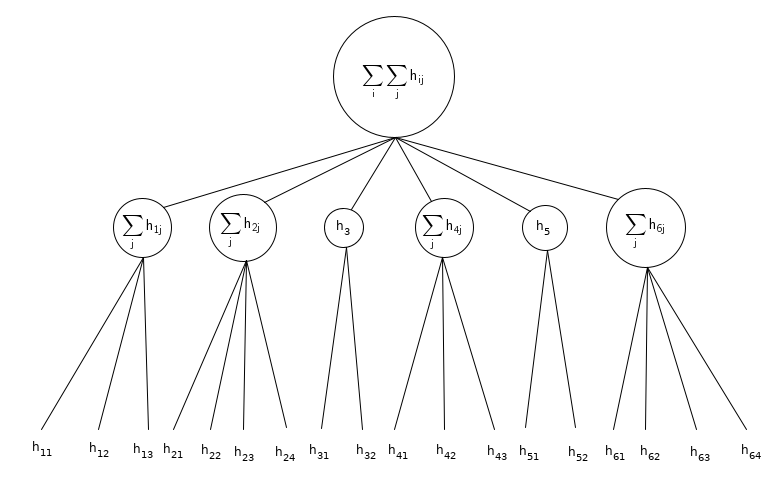
\includegraphics[width=0.8\linewidth]{Screenshot51}
	\caption{Иерархическая структура временных рядов, необходимых для анализа}
	\label{fig:screenshot51}
\end{figure}



\end{frame}


\begin{frame}[shrink=5]
\frametitle{\insertsection} 
\framesubtitle{\insertsubsection}

	\hfil\hfil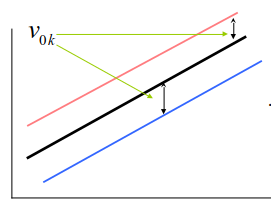
\includegraphics[width=5cm]{screenshot003}\newline
	\null\hfil\hfil\makebox[5cm]{Level 3 residuals}\newline
	\vfil
	\hfil\hfil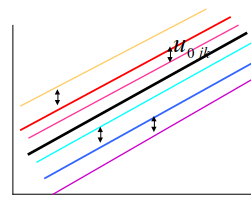
\includegraphics[width=5cm]{screenshot004}\hfil\hfil
	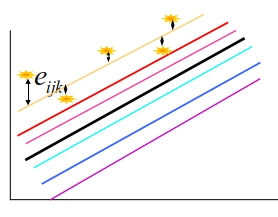
\includegraphics[width=5cm]{screenshot005}\newline
	\null\hfil\hfil\makebox[5cm]{Level 2 residuals}
	\hfil\hfil\makebox[5cm]{Level 1 residuals}

\end{frame}


\subsection{Выбор подходящих наборов данных:} 

\begin{frame}[shrink=5]
\frametitle{\insertsection} 
\framesubtitle{\insertsubsection}


Для анализа были выбраны три набора данных с иерархической структурой с разной сезонностью: 

\begin{itemize}
	\item квартальные (ЕС):
	
	\begin{itemize}
		\item ВВП по 28 странам Европейского союза (включая Великобританию) в разбивке по 10 основным отраслям
		\item Данные собраны за период с 2000-Q1 по 2018-Q3
		\item Источник: Eurostat
	\end{itemize}
	

	\item квартальные сезонно сглаженные (США):
	
	\begin{itemize}
		\item Данные по ВВП США (млн. долл., базовый год 2012) для каждого из 50 штатов с разбивкой по 21 основной отрасли
		\item Данные собраны за период с 2005-Q1 по 2018-Q2
		\item Источник: FRED
	\end{itemize}
		
	\item месячные (РФ):
	
	\begin{itemize}
		\item Данные по смертности и рождаемости в каждом регионе, дающие в сумме естественный прирост населения РФ помесячно
		\item Данные собраны за период с 2006-01 по 2019-01 
		\item Источник: ЕМИСС
	\end{itemize}
		
		
\end{itemize}

\end{frame}



\subsection{US:} 


\begin{frame}[shrink=5]
\frametitle{\insertsection} 
\framesubtitle{\insertsubsection}
	\hfil\hfil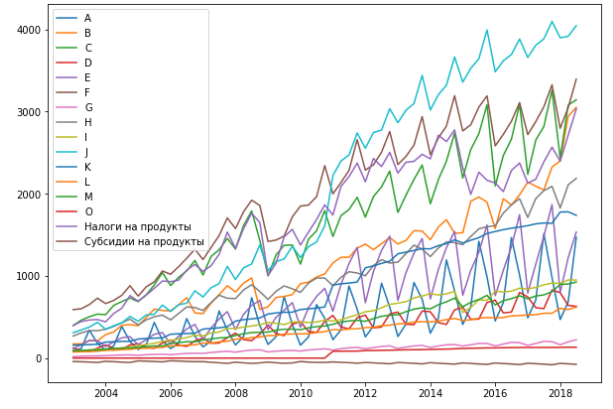
\includegraphics[width=5cm]{screenshot016}\newline
	\null\hfil\hfil\makebox[5cm]{ВВП квартальный (производственный метод):}\newline
	\vfil
	\hfil\hfil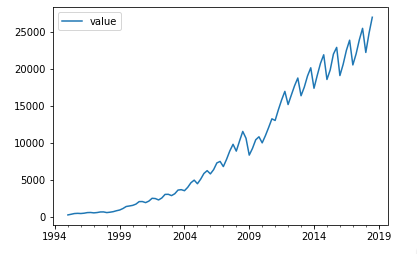
\includegraphics[width=5cm]{screenshot017}\hfil\hfil
	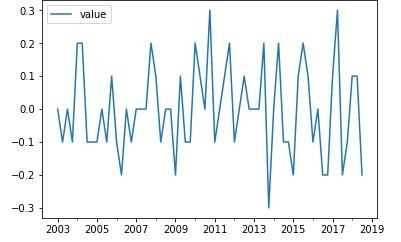
\includegraphics[width=5cm]{screenshot018}\newline
	\null\hfil\hfil\makebox[5cm]{ВВП квартальный}
	\hfil\hfil\makebox[5cm]{Разница (не более 0.00006 \%)}
\end{frame}



\subsection{ЕС:} 

\begin{frame}[shrink=5]
\frametitle{\insertsection} 
\framesubtitle{\insertsubsection}


Квартальные данные по ЕС по секторам: 

2000-01-01 по 2018-07-01


\begin{figure}
	\centering
	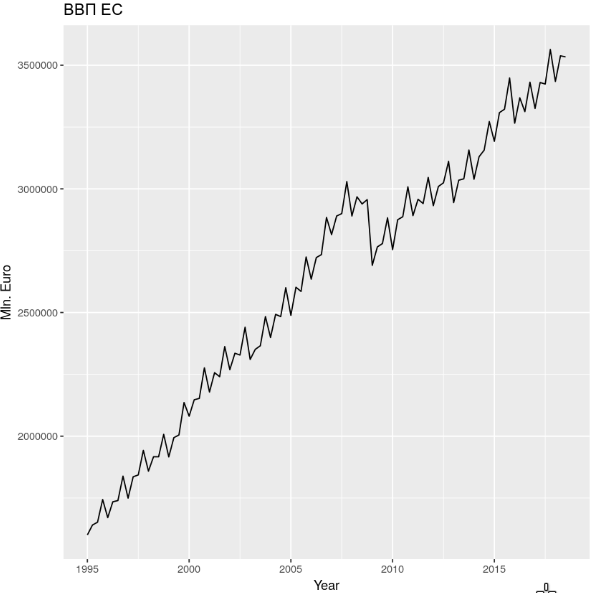
\includegraphics[width=0.7\linewidth]{screenshot021}
	\caption{ВВП ЕС28}
	\label{fig:screenshot021}
\end{figure}





\end{frame}


\section{Forecasting :} 

\subsection{Aggregated TS:} 


\begin{frame}[shrink=5]
\frametitle{\insertsection} 
\framesubtitle{\insertsubsection}



\begin{figure}
	\centering
	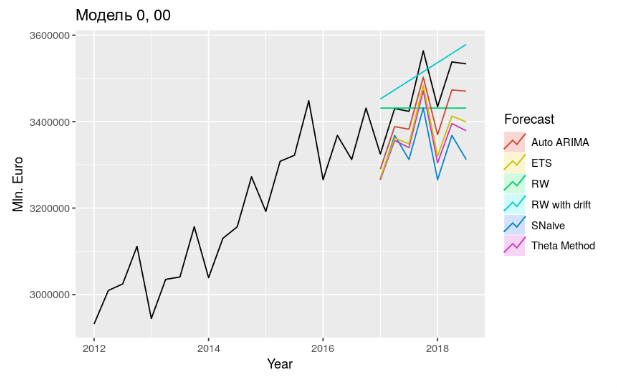
\includegraphics[width=0.7\linewidth]{screenshot022}
	\caption{Сравнение прогнозов}
	\label{fig:screenshot021}
\end{figure}





\end{frame}





\begin{frame}[shrink=5]
\frametitle{\insertsection} 
\framesubtitle{\insertsubsection}



\begin{figure}
	\centering
	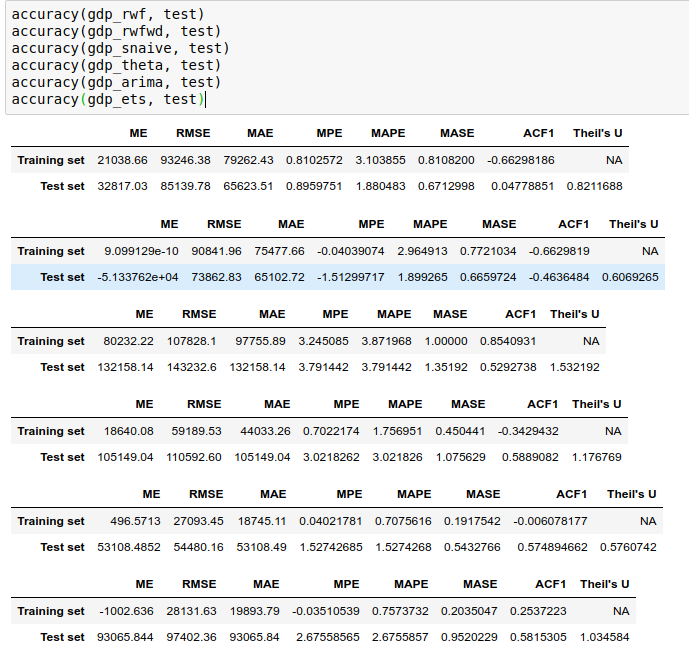
\includegraphics[width=0.7\linewidth]{screenshot023}
	\caption{Сравнение прогнозов}
	\label{fig:screenshot021}
\end{figure}





\end{frame}



\begin{frame}[shrink=5]
\frametitle{\insertsection} 
\framesubtitle{\insertsubsection}

\begin{figure}
	\centering
	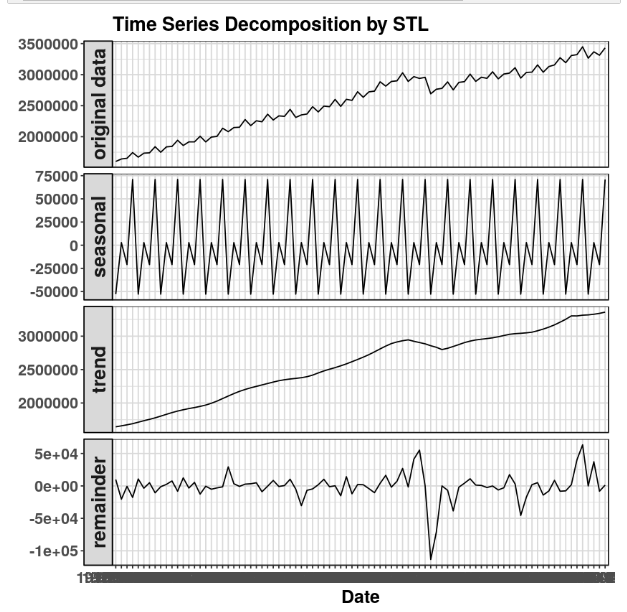
\includegraphics[width=0.7\linewidth]{screenshot024}
%	\caption{}
	\label{fig:screenshot024}
\end{figure}



\end{frame}



\begin{frame}[shrink=5]
\frametitle{\insertsection} 
\framesubtitle{\insertsubsection}

RPART, or CART (Classification and Regression Trees) is recursive partitioning type of binary tree for classification or regression tasks. It performs a search over all possible splits by maximizing an information measure of node impurity, selecting the covariate showing the best split.


\hfil\hfil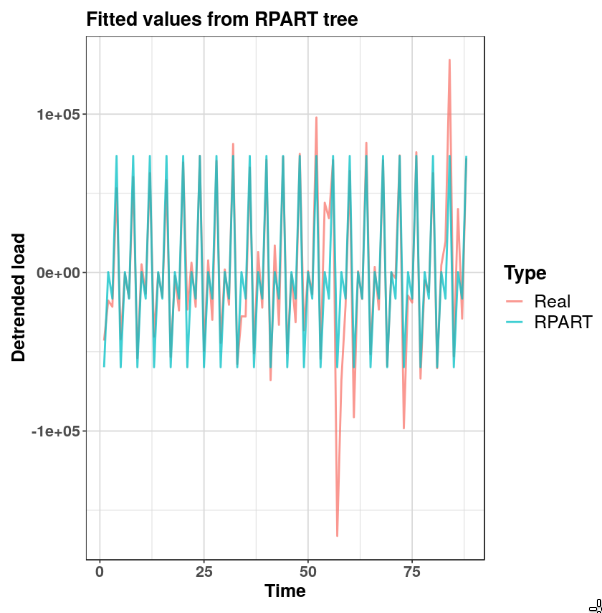
\includegraphics[width=5cm]{screenshot025}\hfil\hfil
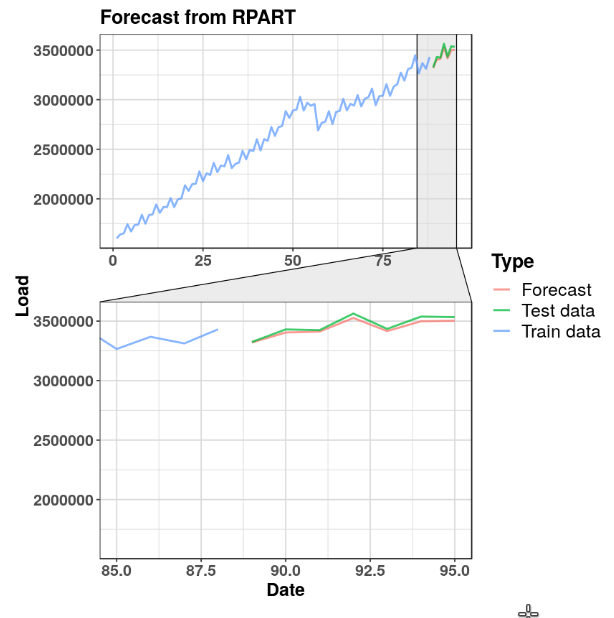
\includegraphics[width=5cm]{screenshot026}\newline
%\null\hfil\hfil\makebox[5cm]{Fit}
%\hfil\hfil\makebox[5cm]{Predict}


%
%\begin{figure}
%	\centering
%	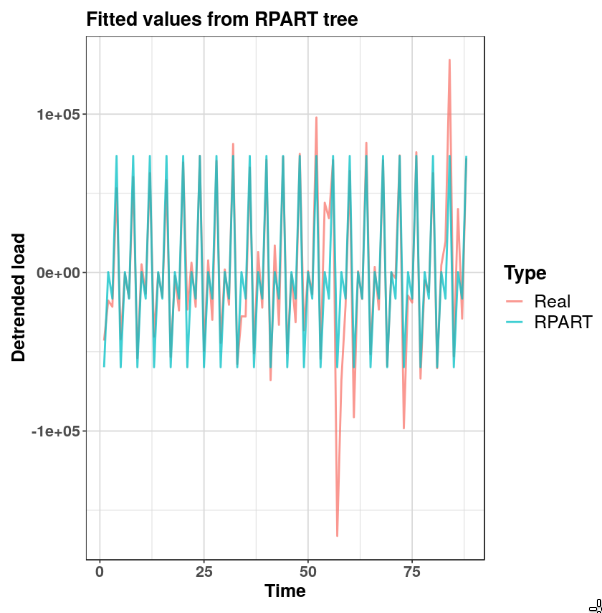
\includegraphics[width=0.7\linewidth]{screenshot025}
%	\caption{}
%	\label{fig:screenshot025}
%\end{figure}


\begin{figure}
	\centering
	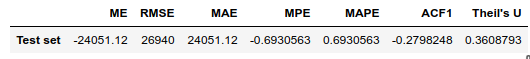
\includegraphics[width=0.7\linewidth]{screenshot027}
	\label{fig:screenshot027}
\end{figure}

\end{frame}



\subsection{Disaggregated TS}


\begin{frame}[shrink=5]
\frametitle{\insertsection} 
\framesubtitle{\insertsubsection}

\begin{figure}
	\centering
	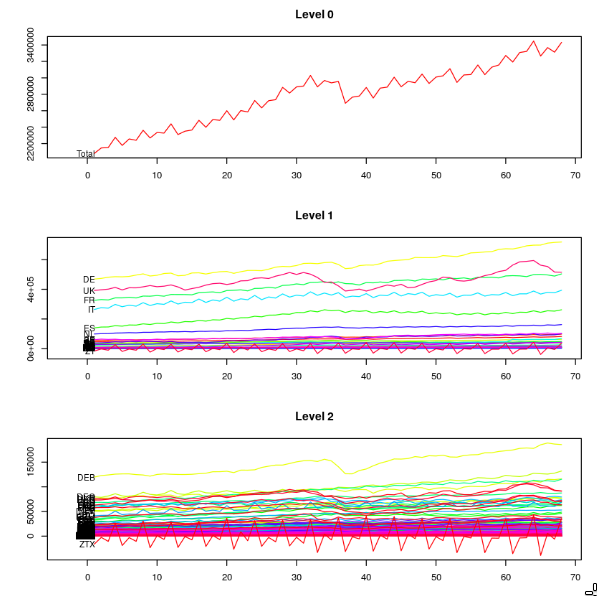
\includegraphics[width=0.7\linewidth]{screenshot028}
%	\caption{}
	\label{fig:screenshot028}
\end{figure}



\end{frame}



\section{Grouped Time Series}



\subsection{Forecasting hierarchical  time series}


\begin{frame}[shrink=5]
\frametitle{\insertsection} 
\framesubtitle{\insertsubsection}



The assumption upon which many of these models are built on, is that by grouping series that behave in a similar way, the idiosyncratic errors within groups will tend to offset each other while the more relevant individual dynamics will be retained to be modelled.



Key idea: forecast reconciliation
\begin{itemize}
	\item Ignore structural constraints and forecast
	every series of interest independently.
	\item Adjust forecasts to impose constraints.
\end{itemize}

Existing methods:
\begin{itemize}
	\item  Bottom-up
	\item  Top-down
	\item  Middle-out
	
\end{itemize}

An “optimal combination” 
approach can be advanced by proposing two new estimators
based on WLS.

Both now implemented in the hts package





\end{frame}



\section{Прогнозирование по рядам второго уровня}
\subsection{Кластеризация временных рядов}



\begin{frame}[shrink=5]
\frametitle{\insertsection} 
\framesubtitle{\insertsubsection}


%
%\begin{figure}
%	\centering
%	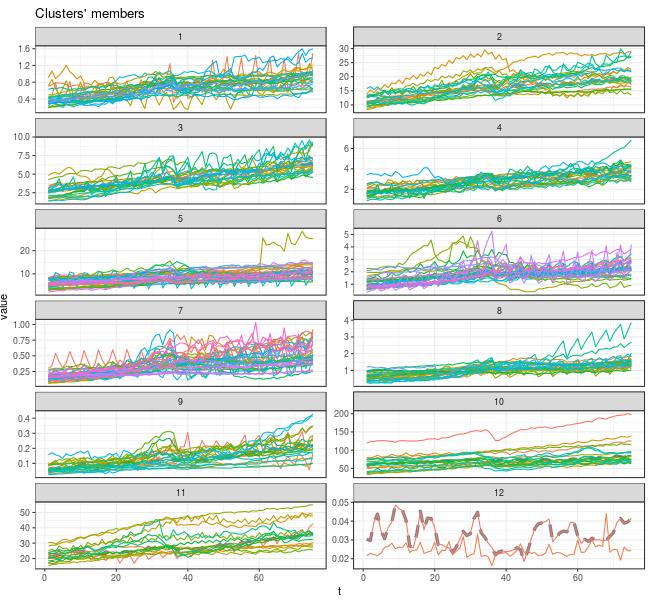
\includegraphics[width=0.7\linewidth]{screenshot047}
%	\caption{}
%	\label{fig:screenshot047}
%\end{figure}
%
%
%\begin{figure}
%	\centering
%	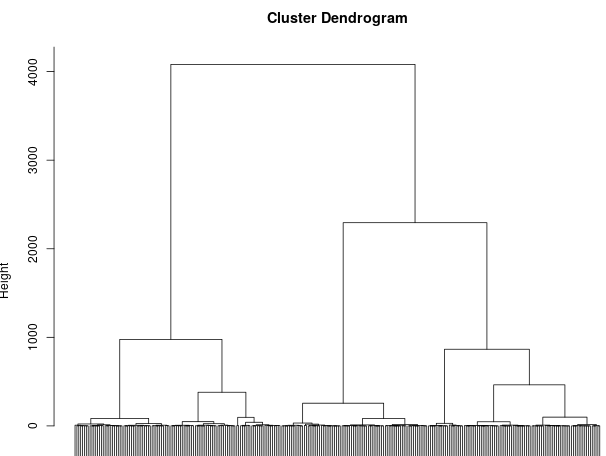
\includegraphics[width=0.7\linewidth]{screenshot046}
%	\caption{}
%	\label{fig:screenshot046}
%\end{figure}

\hfil\hfil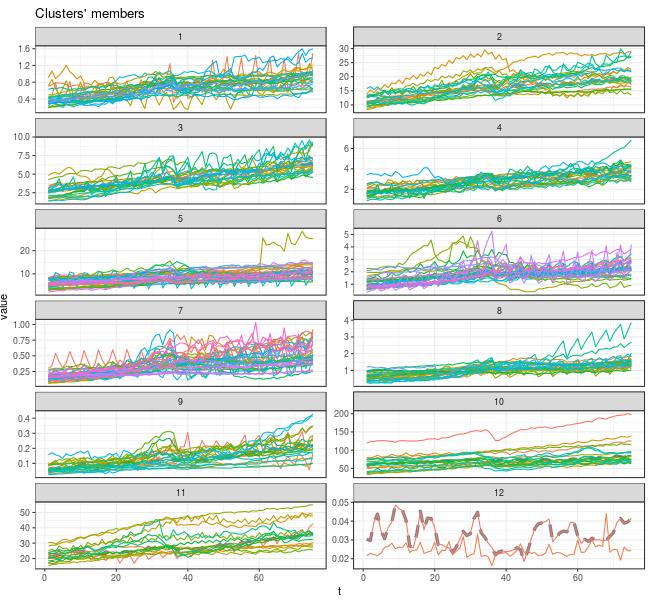
\includegraphics[width=4cm]{screenshot047}\hfil\hfil
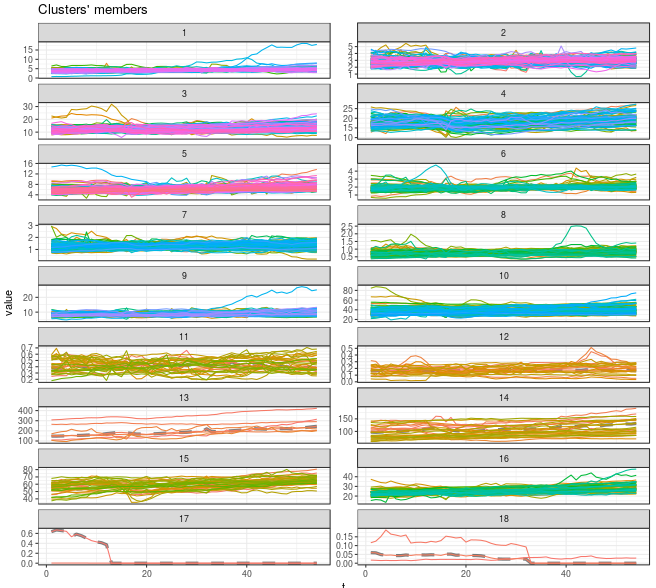
\includegraphics[width=4cm]{screenshot048}\hfil\hfil
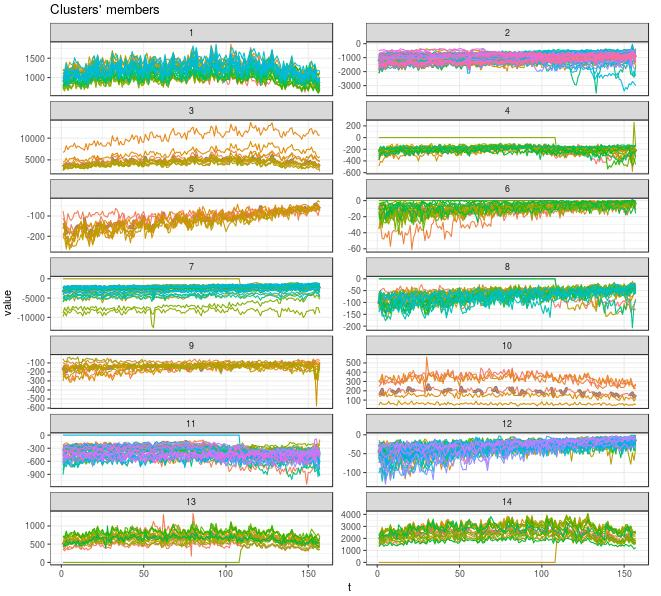
\includegraphics[width=4cm]{screenshot050}\newline

\hfil\hfil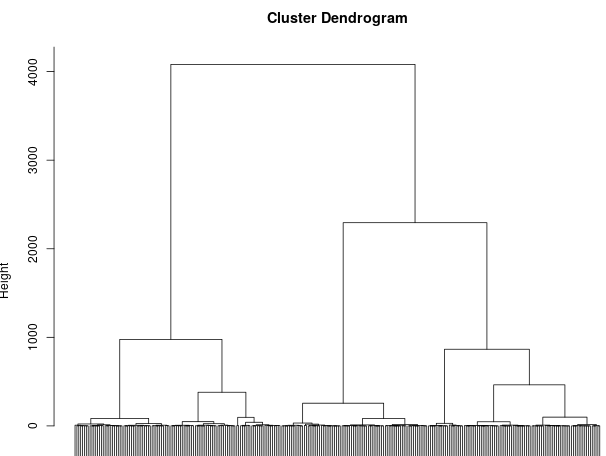
\includegraphics[width=4cm]{screenshot046}\hfil\hfil
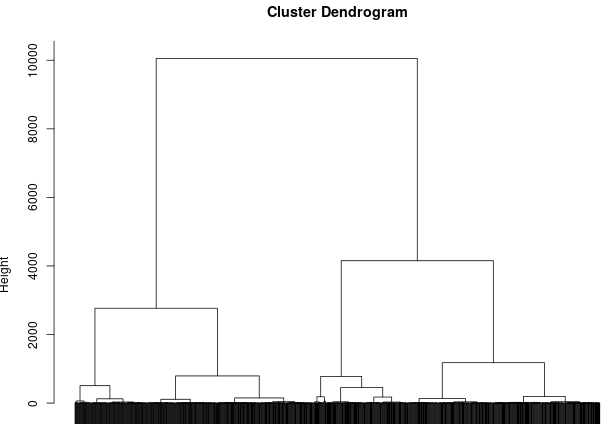
\includegraphics[width=4cm]{screenshot049}\hfil\hfil
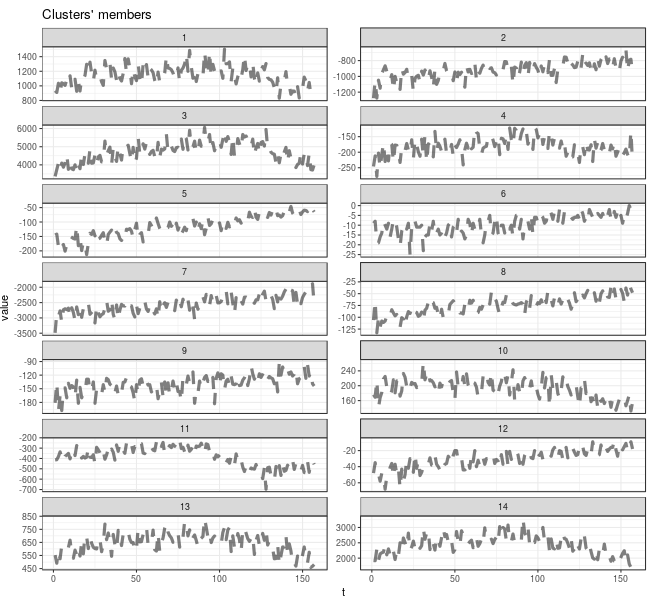
\includegraphics[width=4cm]{screenshot051}\newline




\end{frame}

\section{Сравнение прогнозов}



\begin{frame}[shrink=5]
\frametitle{\insertsection} 
\framesubtitle{\insertsubsection}



\begin{figure}
	\centering
	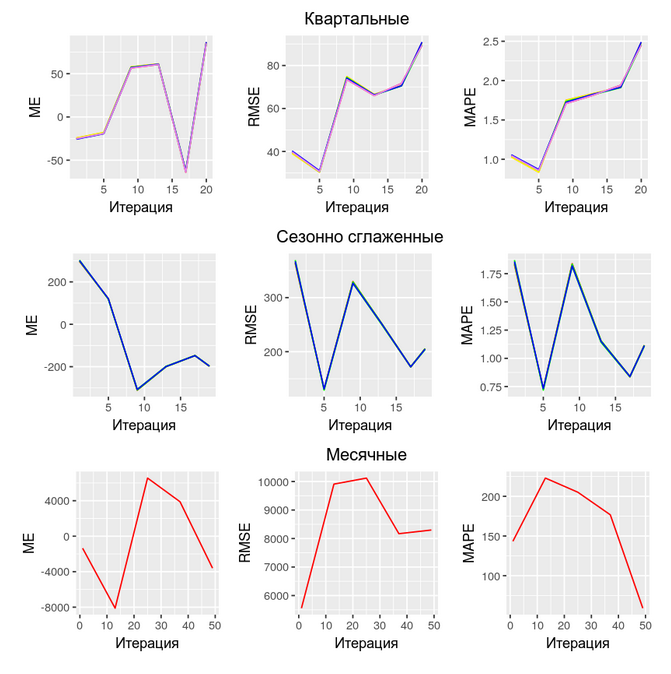
\includegraphics[width=0.7\linewidth]{screenshot052}
	\caption{}
	\label{fig:screenshot052}
\end{figure}




\end{frame}






\begin{frame}[shrink=5]
\frametitle{\insertsection} 
\framesubtitle{\insertsubsection}

\begin{figure}
\centering
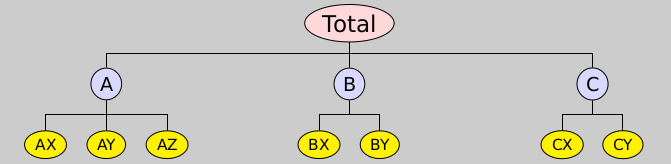
\includegraphics[width=0.7\linewidth]{screenshot010}
\caption{Hierarchical structure}
\label{fig:screenshot010}
\end{figure}


$ Y_t $ : observed aggregate of all
series at time $ t $.

$ Y_{ X , t} $ : observation on series X at
time t.

\end{frame}





\begin{frame}[shrink=5]
\frametitle{\insertsection} 
\framesubtitle{\insertsubsection}


For the hierarchical structure we can write: 

\[\begin{bmatrix}
y_{t} \\
y_{A, t} \\
y_{B, t} \\
y_{AA, t} \\
y_{AB, t} \\
y_{AC, t} \\
y_{BA, t} \\
y_{BB, t}
\end{bmatrix}
=
\begin{bmatrix}
1 & 1 & 1 & 1 & 1 \\
1 & 1 & 1 & 0 & 0 \\
0 & 0 & 0 & 1 & 1 \\
1  & 0  & 0  & 0  & 0  \\
0  & 1  & 0  & 0  & 0  \\
0  & 0  & 1  & 0  & 0  \\
0  & 0  & 0  & 1  & 0  \\
0  & 0  & 0  & 0  & 1
\end{bmatrix}
\begin{bmatrix}
y_{AA, t} \\
y_{AB, t} \\
y_{AC, t} \\
y_{BA, t} \\
y_{BB, t}
\end{bmatrix}\]


or in more compact notation,  where  $y_t$   is an $n$-dimensional vector of all the observations in the hierarchy at time $t$, $S$  is the summing matrix.

$$y_t  = S b_t$$


$ b_t $ : $m$-dimensional vector of all series at
bottom level in time t.


\end{frame}









\begin{frame}[shrink=5]
\frametitle{\insertsection} 
%\framesubtitle{\insertsubsection}

%\begin{figure}
%	\centering
%	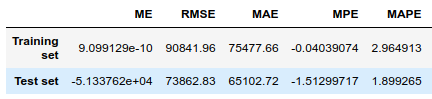
\includegraphics[width=0.7\linewidth]{screenshot031}
%	\caption{}
%	\label{fig:screenshot031}
%\end{figure}
%
%
%\begin{figure}
%	\centering
%	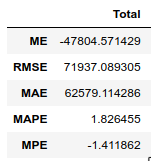
\includegraphics[width=0.7\linewidth]{screenshot030}
%	\caption{}
%	\label{fig:screenshot030}
%\end{figure}

\hfil\hfil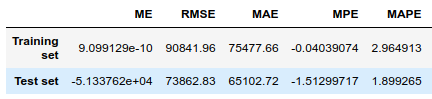
\includegraphics[width=5cm]{screenshot031}\hfil\hfil
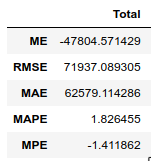
\includegraphics[width=1.5cm]{screenshot030}\newline


\hfil\hfil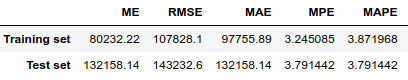
\includegraphics[width=5cm]{screenshot039}\hfil\hfil
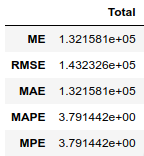
\includegraphics[width=1.5cm]{screenshot033}\newline

\hfil\hfil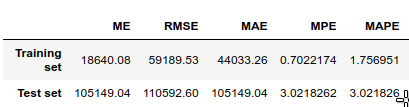
\includegraphics[width=5cm]{screenshot040}\hfil\hfil
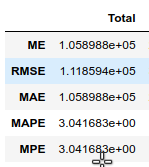
\includegraphics[width=1.5cm]{screenshot035}\newline


\hfil\hfil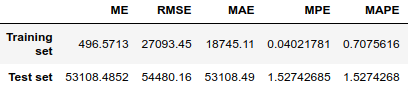
\includegraphics[width=5cm]{screenshot041}\hfil\hfil
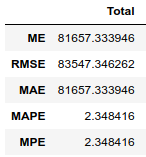
\includegraphics[width=1.5cm]{screenshot036}\newline


\end{frame}




\subsection{ARIMAX}




\subsection{Forecasting 	grouped time series}



\begin{frame}[shrink=5]
\frametitle{\insertsection} 
\framesubtitle{\insertsubsection}




\[\begin{bmatrix}
y_{t} \\
y_{A, t} \\
y_{B, t} \\
y_{X, t} \\
y_{Y, t} \\
y_{AA, t} \\
y_{AB, t} \\
y_{AC, t} \\
y_{BA, t} \\
y_{BB, t}
\end{bmatrix}
=
\begin{bmatrix}
1 & 1 & 1 & 1 & 1 \\
1 & 1 & 1 & 0 & 0 \\
0 & 0 & 0 & 1 & 1 \\
1 & 0 & 1 & 0 & 1 \\
0 & 1 & 0 & 1 & 0 \\
1  & 0  & 0  & 0  & 0  \\
0  & 1  & 0  & 0  & 0  \\
0  & 0  & 1  & 0  & 0  \\
0  & 0  & 0  & 1  & 0  \\
0  & 0  & 0  & 0  & 1
\end{bmatrix}
\begin{bmatrix}
y_{AA, t} \\
y_{AB, t} \\
y_{AC, t} \\
y_{BA, t} \\
y_{BB, t}
\end{bmatrix}\]


\begin{figure}
	\centering
	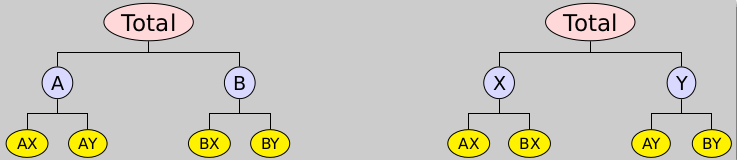
\includegraphics[width=0.7\linewidth]{screenshot011}
	\caption{Grouped structure}
	\label{fig:screenshot011}
\end{figure}


\end{frame}





\subsection{Optimal forecasts}

\begin{frame}[shrink=5]
\frametitle{\insertsection} 
\framesubtitle{\insertsubsection}

\[ \hat{Y}_n ( h ) = S \beta_n ( h ) + e_h  \]

$ \hat{Y}_n ( h ) $ - a vector of initial $ h $-step forecasts,
made at time $ n $, stacked in same order as $ Y_t  $.

$ \beta_n ( h )   = E [ B _{n + h} | Y_1 , \dots , Y_n ]  $

$ e_h  $  has zero mean and covariance $ \Sigma_h  $.

\[ \tilde{Y}_n ( h )
= S \hat{\beta}_n ( h ) = S P  \hat{Y}_n ( h ) =  S ( S' \Sigma^{+}_h S )^{-1}  S'  \Sigma^{+}_h  \hat{Y}_n ( h )
 \]
 
$ \tilde{Y}_n ( h ) $   - revised forecasts, 
$ \hat{Y}_n ( h ) $ - initial forecasts

$ \Sigma^{+}_h $ - generalized inverse of $ \Sigma_h $.

Optimal $ P = ( S' \Sigma^{+}_h S )^{-1}  S'  \Sigma^{+}_h  $

Problem: $ \Sigma_h $ hard to estimate.

\end{frame}



\subsection{Approximate optimal forecasts}



\begin{frame}[shrink=5]
\frametitle{\insertsection} 
\framesubtitle{\insertsubsection}


\[ \tilde{Y}_n ( h )
= 
 S ( S' \Sigma^{+}_h S )^{-1}  S'  \Sigma^{+}_h  \hat{Y}_n ( h )
\]


\begin{itemize}
	\item OLS
	
 	 $ e_{B , h} $ is the forecast
	error at bottom level.
	
	Assume $ e_h \approx S e_{B , h} $ 	
	then $ ( S' \Sigma^{+}  S )^{-1} S'  \Sigma^{+} = ( S'S )^{ - 1} S'  $
	
	
\[  \tilde{Y}_n ( h )
 =  S ( S'  S )^{-1}  S'   \hat{Y}_n ( h )
 \]	
	
	
	\item Rescaling
	
	Suppose we approximate $ \Sigma_h $ by its diagonal: 
$ \Lambda = diag(\hat{\Sigma}_1)^{-1}
 $,  which	
 contain inverse
	one-step ahead in-sample forecast error
	variances.
	
	\[ \tilde{Y}_n ( h )
	=  S ( S'  \Lambda S )^{-1}  S'   \Lambda  \hat{Y}_n ( h )
	\]
	
	\item Averaging
	
	If the bottom level error series are
	approximately uncorrelated and have similar
	variances, then $ \Lambda $ is inversely proportional to
	the number of series contributing to each
	node: 
	$ \Lambda = diag( S \times 1 )^{- 1}
 $ is  the inverse row sums of S
 
\end{itemize}




\end{frame}






\section{Clusterization methods}

\section{Forecast-error clustering}


\begin{frame}[shrink=5]
\frametitle{\insertsection} 
\framesubtitle{\insertsubsection}


\begin{figure}
	\centering
	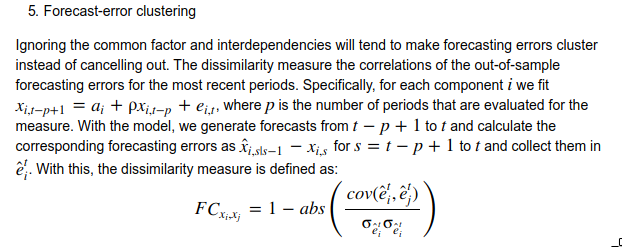
\includegraphics[width=0.7\linewidth]{screenshot043}
	%	\caption{RW with drift}
	\label{fig:screenshot029}
\end{figure}


\end{frame}








\section{Bayesian Methods}





\subsection{Why is the Bayesian Inference controversial?}

\begin{frame}[shrink=5]
\frametitle{\insertsection} 

\textbf{Forward	modelling:	}   with
  noise	
properties	
  we	
 can	 predict	
  the	Sampling	
  
Distribution
   (the probability	
  for	
  a	
 general	
  set	
  of	
 data


In	
  easy	
  cases,	
  the	
  effect	
  of	
  the	
  prior	
  is	
  simple. As	
  experiment	
  gathers	
  more	
  data,	
  the	
  likelihood	
  tends	
  to	
  get	
  narrower,	
  and	
  the	
  influence	
  of	
  the	
  prior	
  diminishes.	
  

Rule	
  of	
  thumb:	
  if	
  changing	
  your	
  prior	
  to	
  another	
  reasonable	
 one	
  changes	
  the	
  answers	
  significantly,	
  you	
  need	
  more	
  data	
  



\end{frame}





\begin{frame}[shrink=5]
\frametitle{\insertsection} 
\framesubtitle{\insertsubsection}


\begin{enumerate}
	\item  Bayesians claim that the parameters are random so that their credible interval is a valid probability argument, though it also depends on the  the prior, which is usually hard to obtain.
	
	\item When the likelihood and prior is complicated, the inference has to rely on the MCMC sampling, which can be really slow in most of the real-world cases.

	\item  The biggest controversy about Bayesian inference is that you must quantify your prior knowledge about the question at hand. This makes it possible to actually influence your results, either accidentally or on purpose. 	
\end{enumerate}
\end{frame}






\subsection{Bayesian Modelling and Markov chain Monte Carlo}


\begin{frame}[shrink=5]
\frametitle{\insertsection} 
\framesubtitle{\insertsubsection}

Bayesian method provides an intuitive way for us to fill the gaps left by small or incomplete data sets. 


To calculate the Bayesian predictive distribution, $\pi(x|D)$, given some data $D$,  we simply multiply the density function of the classical solution  $\ell (D|x)$,  with the density function produced by our prior knowledge $\pi(x)$. This is a direct application of Bayes’ theorem. Unfortunately, this product will not integrate to one. To overcome this, we multiply the density function by a constant $Z$, which rescales the density so that it does integrate to one. The resulting Bayesian distribution defined over the n-dimensional parameter space $S$ is

$$ \pi(x|D) = \frac{1}{Z} \pi(x) \ell(D|x)$$

$$ Z = \int_S \pi(x) \ell(D|x) dx$$

In one dimension it is easy to use numerical quadrature to calculate $Z$. However as the dimension becomes large, this method quickly becomes impractical. So we turn to a class of statistical algorithms known as Markov chain Monte Carlo (MCMC) methods, which can tackle these high dimensional parameter spaces.



\end{frame}





\subsection{Bayesian Shrinkage}


\begin{frame}[shrink=5]
\frametitle{\insertsection} 
\framesubtitle{\insertsubsection}

\textbf{Shrinkage} is implicit in Bayesian inference and penalized likelihood inference, and explicit in James–Stein-type inference. In contrast, simple types of maximum-likelihood and least-squares estimation procedures do not include shrinkage effects, although they can be used within shrinkage estimation schemes.
 
 
 
\end{frame}

\subsection{Stein's  paradox}


\begin{frame}[shrink=5]
\frametitle{\insertsection} 
\framesubtitle{\insertsubsection}
 
 
\textbf{Stein's  paradox}, in decision theory and estimation theory, is the phenomenon that when three or more parameters are estimated simultaneously, there exist combined estimators more accurate on average (that is, having lower expected mean squared error) than any method that handles the parameters separately. 

\textit{The best guess about the future is usually  obtained by computing the average of past events. Stein's paradox defines circumstances in which there are estimators better that the arithmetic average
}

Stein’s paradox  **modern generalization, the Bayesian hierarchical model**. 

Bayesian hierarchical model can improve overall estimation accuracy, thereby improving our confidence in the assessment results, especially for standard compliance assessment of waters with **small sample sizes.**


\end{frame}
 
\section{MCMC}
 
 
\section{Hierarchical Bayes}




\section{Small Sample}

\begin{frame}[shrink=5]
\frametitle{\insertsection} 


Most of the inferential procedures available in the analysis of time series data are asymptotic

Although analytic small sample results are available in a few cases, there is currently, no widely applicable and easily accessible method that can be used to make small sample inferences.

\end{frame}



\section{Bootstrap}




\begin{frame}[shrink=5]
\frametitle{\insertsection} 


The bootstrap technique introduced by Efron (1979) could possibly be a potential alternative in estimation and inference from time series models in finite samples. However, in time series regressions, the standard bootstrap resampling method designed for independent and identically distributed (IID) errors is not applicable because in most situations the assumption of IID errors is violated. 


The basic bootstrap approach consists of drawing repeated samples (with replacement). 
The simplest assumption for that method is that observations should be IID. 
But in time series models IID assumption is not satisfied.
Thus the method needs to be modified.

	\begin{block}{BS for TS:}

\begin{itemize}
	\item Estimating Standard Errors:  if “Small Sample Size” distribution is normal then we can get a BS distribution to Estimate SE (same as asymptotic distribution for SE)
	\item Confidence Interval statements:
	Using BS distribution to Estimate CI we can get  different result for CI (from asymptotic distribution), for example, because of BS distribution skewness 
\end{itemize}

\end{block}

\end{frame}




\subsection{The Recursive BS for stationary AR(p) model}

\begin{frame}[shrink=5]
\frametitle{\insertsection} 
\framesubtitle{\insertsubsection}


Consider AR(p) process:
\[ y_t = \sum_{i=1}^p a_i y_{t-i} + e_t, e_t \sim N(0,\sigma^2)\]

We estimate coefficients with OLS and get: 
\[ (\hat{a}_1,\dots, \hat{a}_p), \hat{e}_t \]




 Define the centered and scaled residuals:
\[ \tilde{e}_t = (\hat{e}_{t} - \frac{1}{n} \sum \hat{e}_{t} )  \left( \frac{n}{n-p}\right) ^{1/2} \]
Resample $ \tilde{e}_t $ with replacement to get the BS residuals $ e_t^* $

Construct the BS sample recursively using $ y_t^* = y_t $:

\[ y_t^* = \sum_{i=1}^p \hat{a}_i y_{t-i}^* + e_t^*\]


\end{frame}


\subsection{A comparison of four different block bootstrap methods}

\begin{frame}[shrink=5]
\frametitle{\insertsection} 
\framesubtitle{\insertsubsection}




\begin{figure}
	\centering
	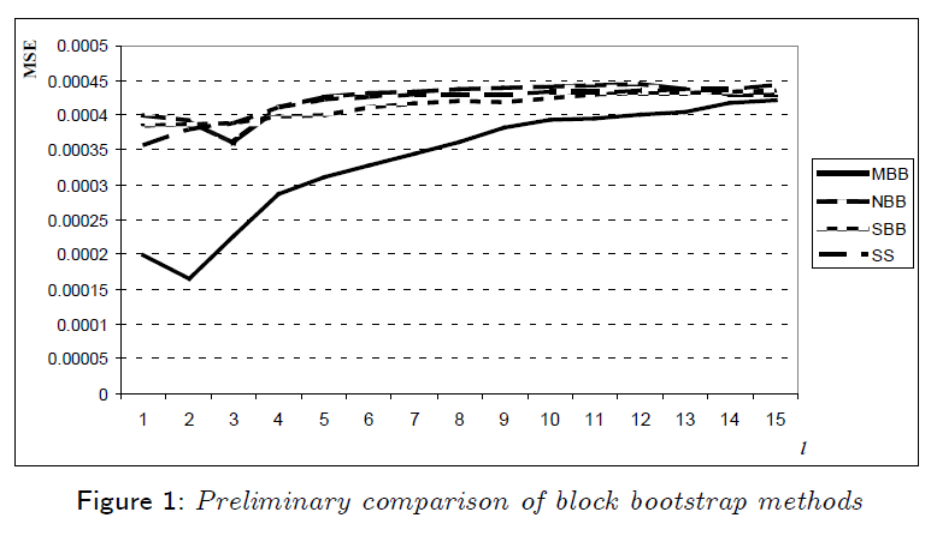
\includegraphics[width=0.7\linewidth]{screenshot008}
	\caption{MBB – Moving block bootstrap, 
		NBB – Non-overlapping block bootstrap, 
		SBB – Stationary block bootstrap, 
		SS - Subsampling }
	\label{fig:screenshot008}
\end{figure}

\end{frame}




\subsection{Bootstrapping vs. Posterior sampling}

\begin{frame}[shrink=5]
\frametitle{\insertsection} 
\framesubtitle{\insertsubsection}

“Bootstrapping” is a a framework that aims to improve simple but approximate frequentist methods:

\begin{itemize}
	\item Parametric bootstrap: Improve asymptotic behavior of
estimates for a trusted model: reduce bias of estimates,
provide more accurate coverage of confidence regions

\item Nonparametric bootstrap: Provide results that are
approximately accurate with weak modeling assumptions

\end{itemize}

Most common approach uses Monte Carlo to simulate an ensemble
of data sets related to the observed one, and use them to
recalibrate a simple method.

Parametric bootstrap has a step producing an ensemble of
estimates that looks like a set of posterior samples. Can they be
thought of this way?

\end{frame}






















\end{document}